\subsection{Auswertung der Promptkurve}

\begin{figure}[h]
\centering
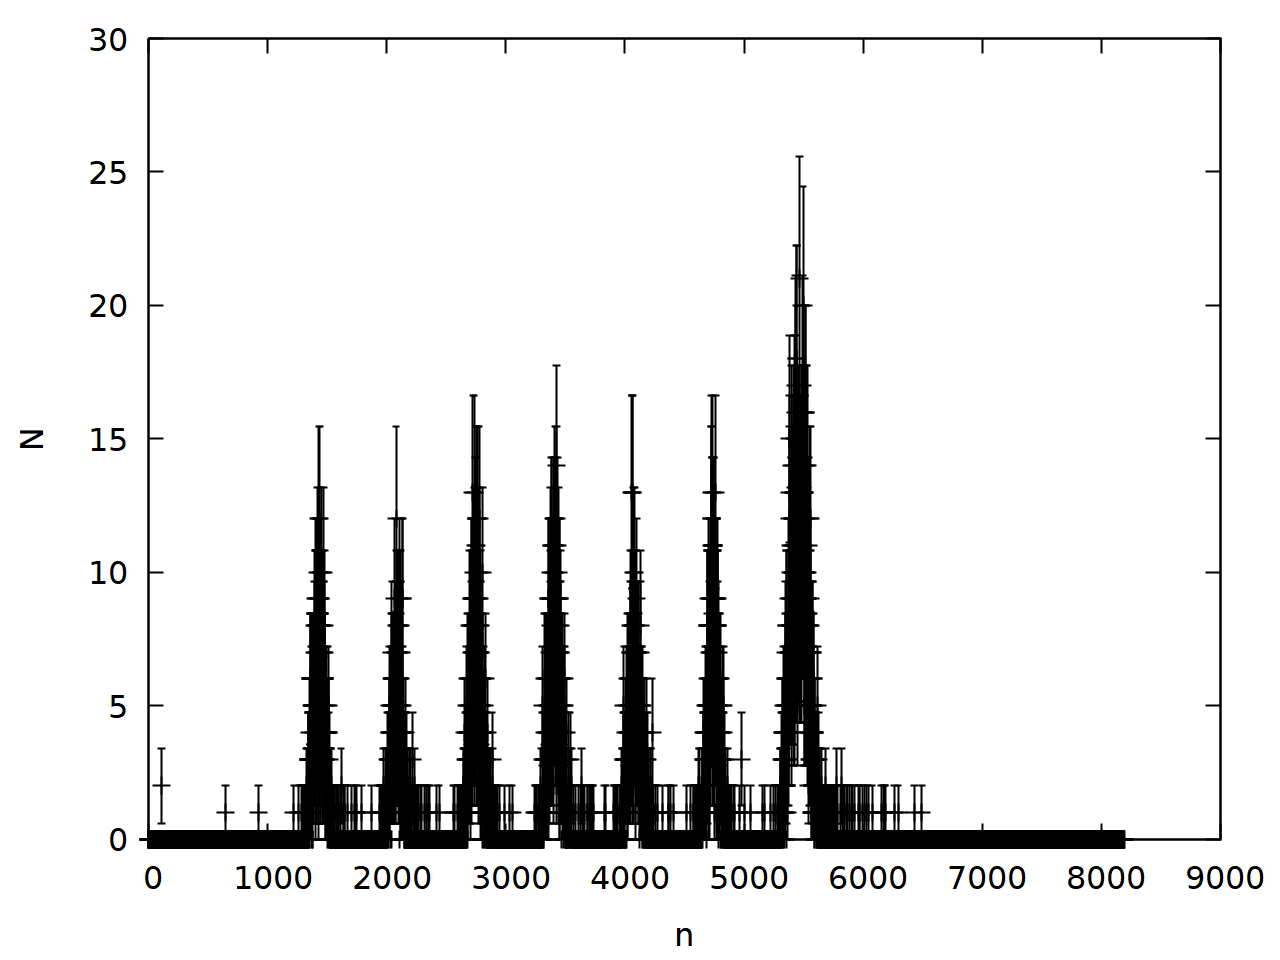
\includegraphics[width=0.7\linewidth]{data/prompt.png}
\caption{Gemessene Promptkurve}
\label{fig:prompt}
\end{figure}

\begin{figure}[h]
\centering
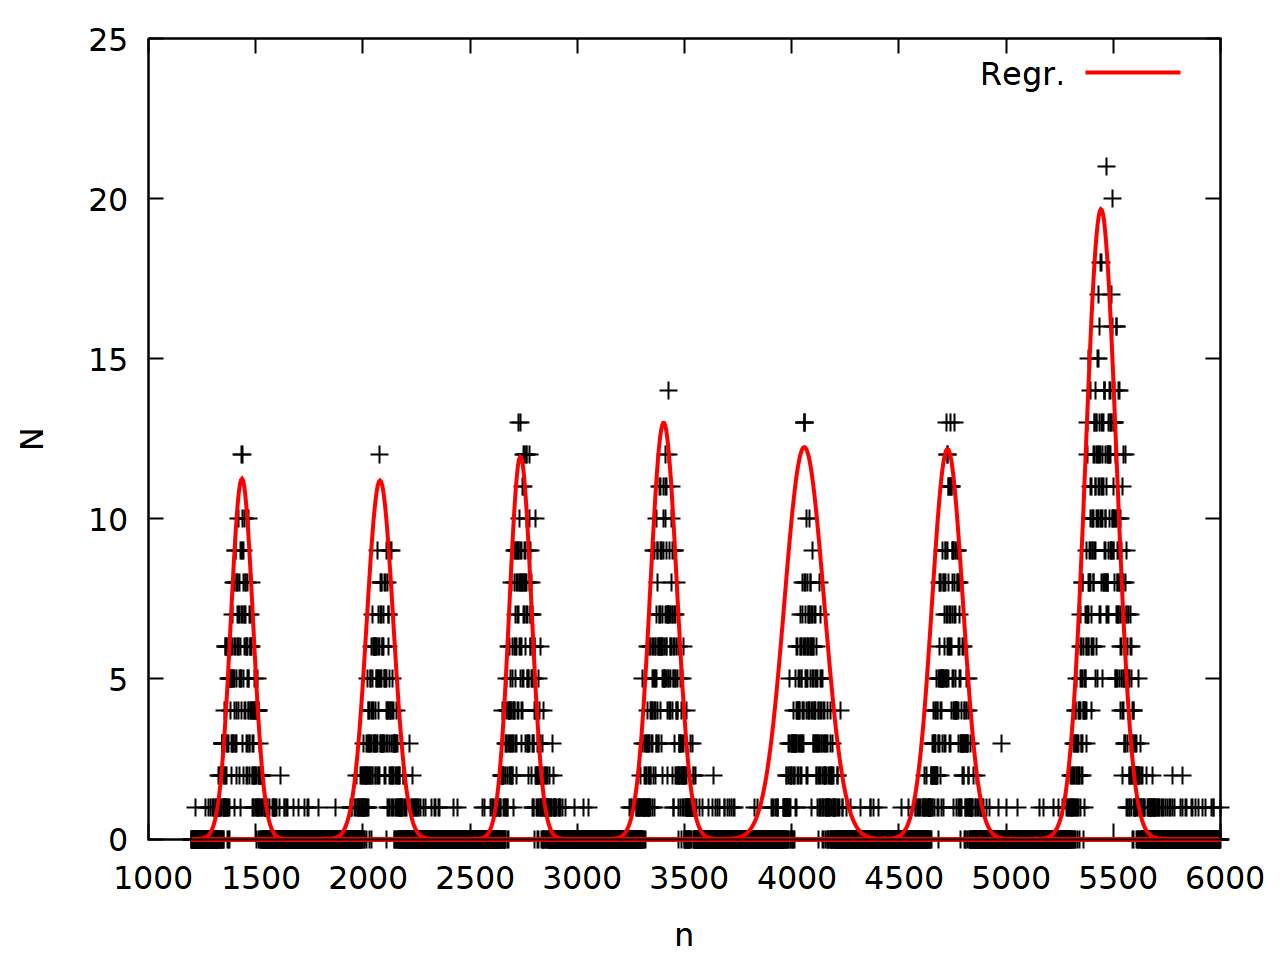
\includegraphics[width=0.7\linewidth]{data/prompt2.png}
\caption{Promptkurve mit Fits}
\label{fig:prompt2}
\end{figure}

In Abb. \ref{fig:prompt} ist die gemessene Promptkurve zu sehen. An die einzelnen Peaks wird nun jeweils eine Gausskurve \[f(x) = a\exp{\left(-\frac{(x-n)^2}{2\sigma^2}\right)}\]mit Fityk gefittet. Das Ergebnis ist in Tab. \ref{tab:prompt} aufgelistet und in Abb. \ref{fig:prompt2} mit den Daten abgebildet.

\begin{table}[h]
\centering
\caption{Fitergebnisse für die Gausskurven}
\label{tab:prompt}
\begin{tabular}{cccc}
\toprule
Peak Nr. & a & n & $\sigma$\\
\midrule
6&	19,67&	5443&	72,19\\
5&	12,18&	4727&	72,19\\
4&	12,24&	4059&	92,58\\
3&	13&	3403&	62\\
2&	11,95&	2735&	51,81\\
1&	11,2&	2080&	62\\
0&	11,25&	1436&	51,81\\
\bottomrule
\end{tabular}
\end{table}

Der Abstand der Peaks entspricht jeweils \SI{16}{\nano\second}. Um zu bestimmen, wie vielen Bins diese \SI{16}{\nano\second} entsprechen wird die Position des Peaks über der Peaknummer multipliziert mit \SI{16}{\nano\second} aufgetragen (siehe Abb. \ref{fig:prompt_time}). Als Fehler der Peakpositionen wird die Standartabweichung $\sigma$ angenommen.  

\begin{figure}[h]
\centering
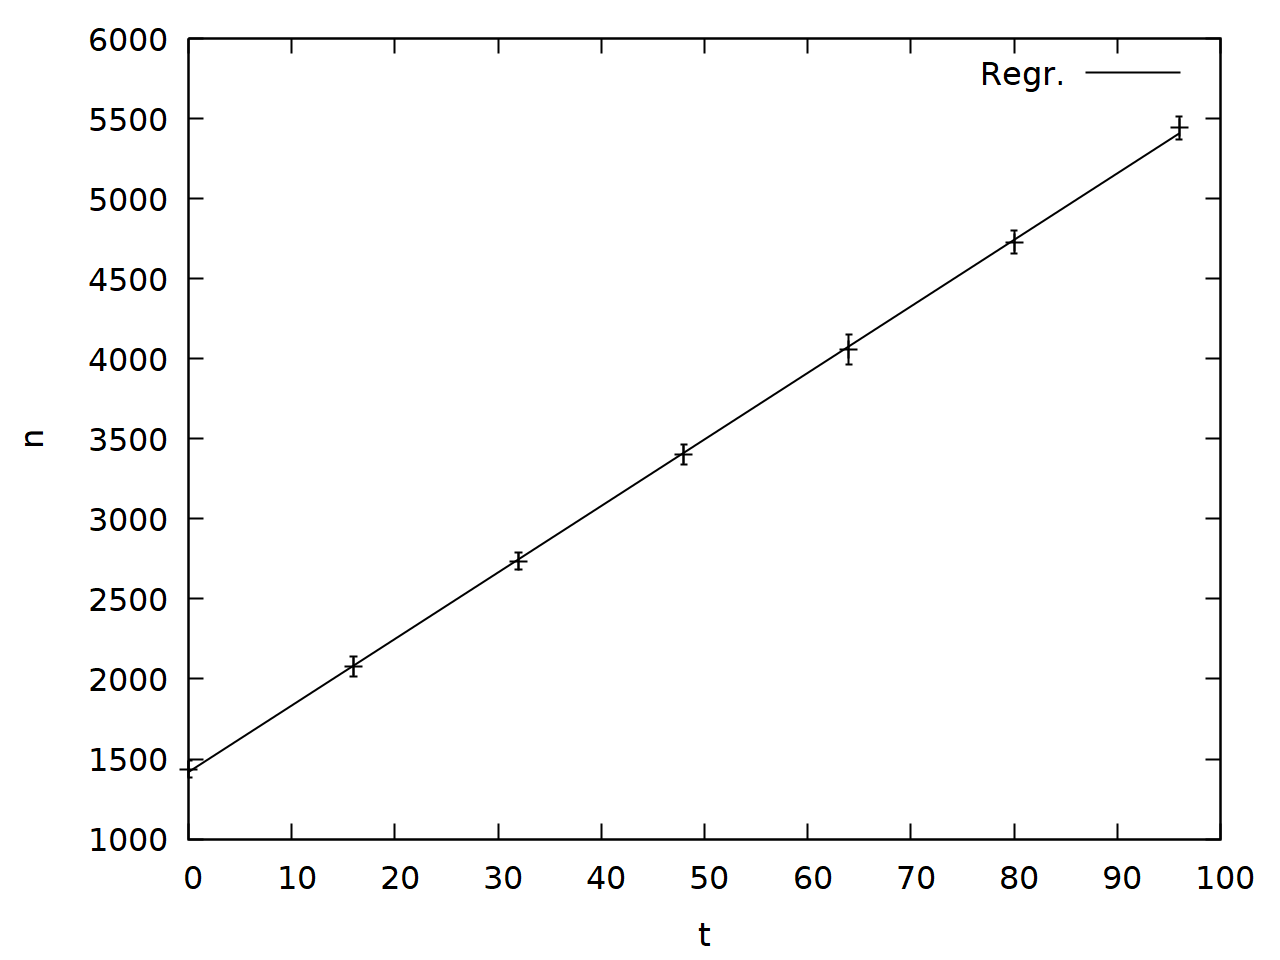
\includegraphics[width=0.7\linewidth]{data/prompt_time.png}
\caption{Positionen der Peaks über der Zeit}
\label{fig:prompt_time}
\end{figure}

Ein linearer Fit $a\cdot t + b$ ergibt:\\
\begin{align*}
a &= (41,5 \pm 0,2) \si{\nano\second}^{-1}\\
b &= (1,42 \pm 0,01) \cdot 10^{3}\\
\end{align*}

Das bedeutet, dass \SI{16}{\nano\second} 41,5 Bins entsprechen.

\subsection{Bestimmung der Lebensdauer}

\begin{figure}[h]
\centering
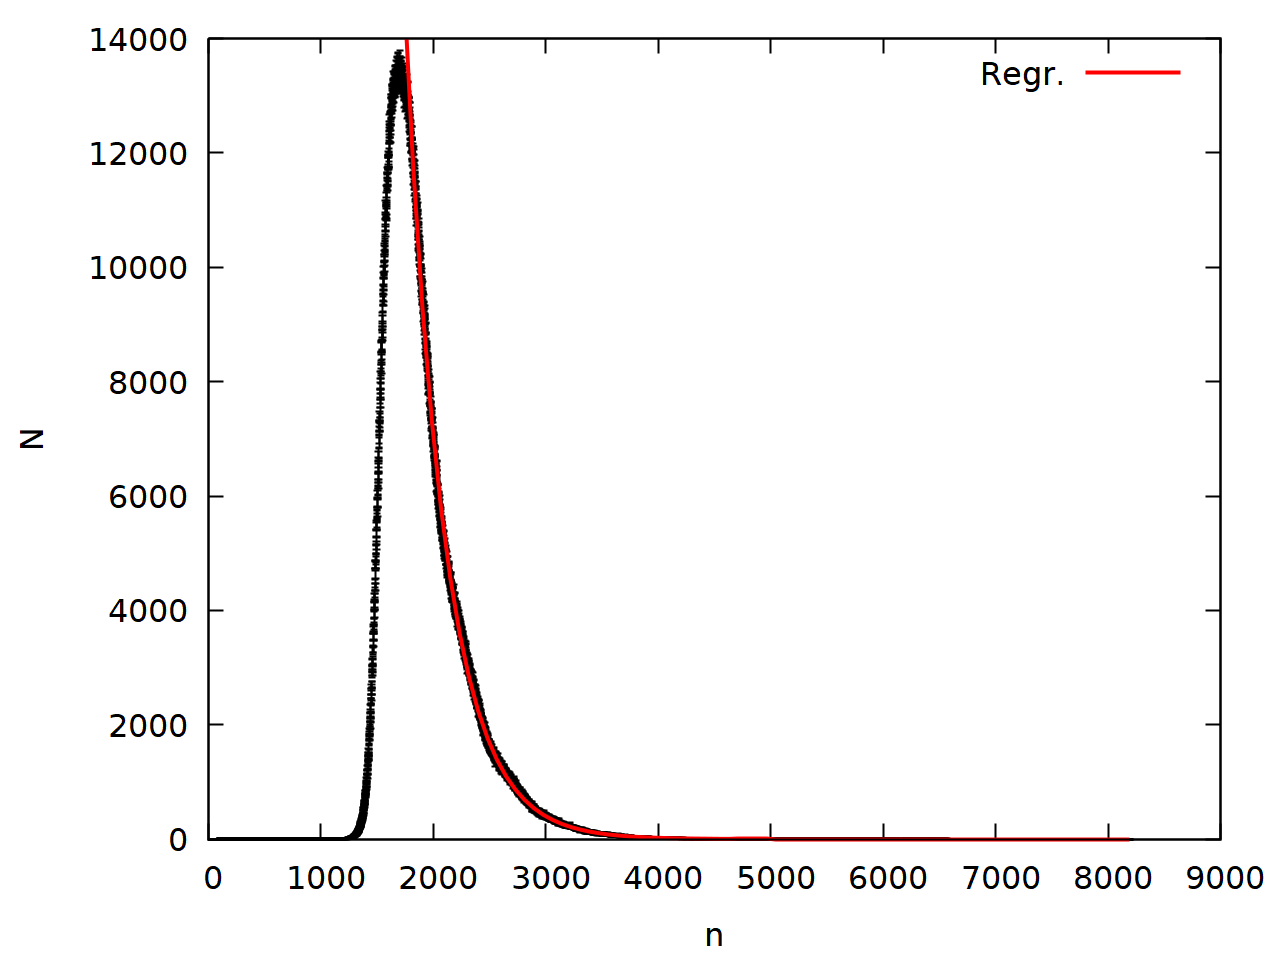
\includegraphics[width=0.7\linewidth]{data/uebernacht.png}
\caption{Ergebnis der Lebensdauermessung}
\label{fig:halflife}
\end{figure}

\begin{figure}[h]
\centering
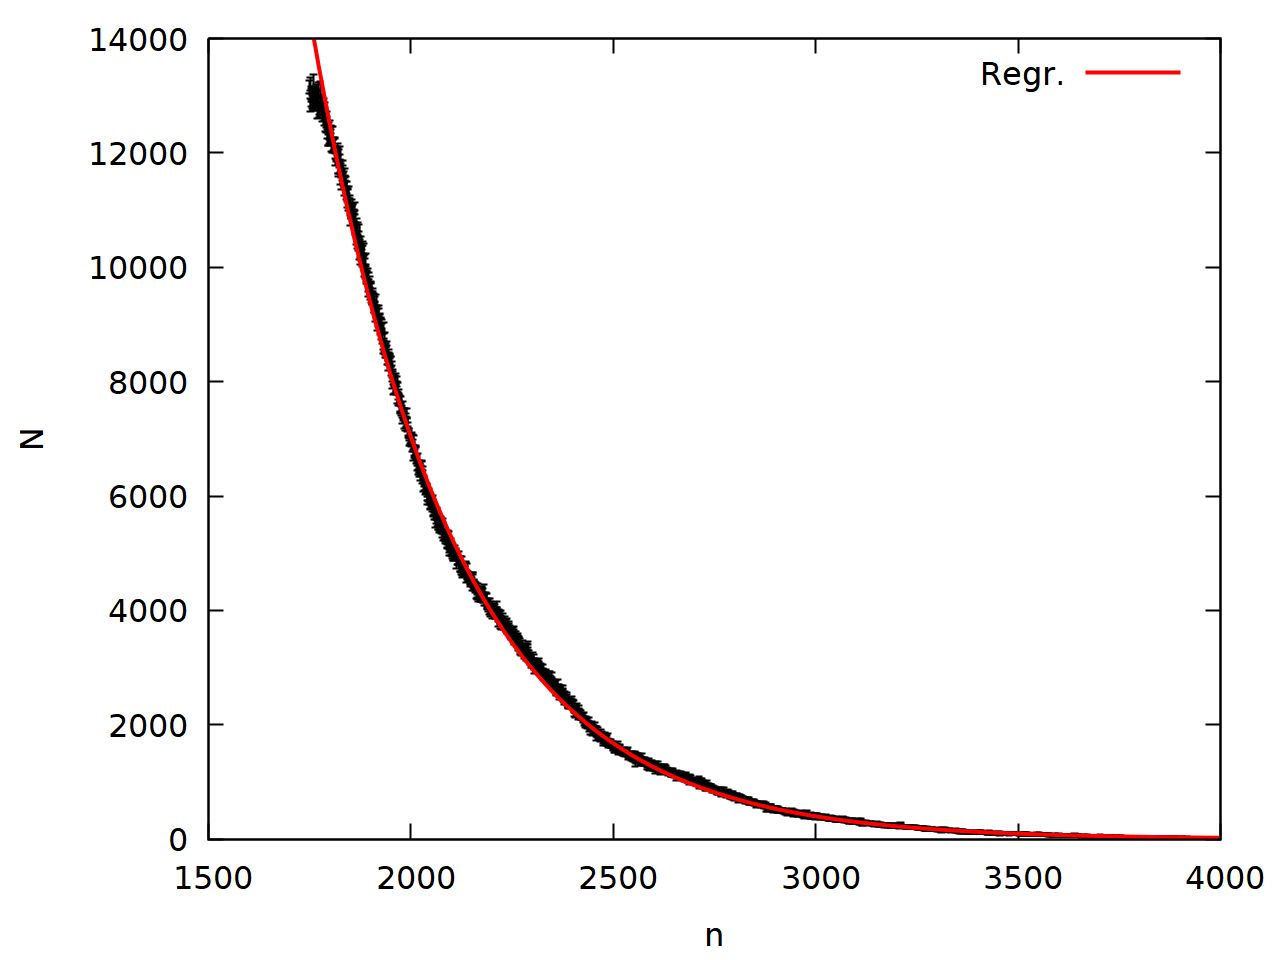
\includegraphics[width=0.7\linewidth]{data/uebernacht2.png}
\caption{Exponentieller Fit an die Lebensdauermessung}
\label{fig:halflife2}
\end{figure}

In Abb. \ref{fig:halflife} sind die gemessenen Ereignisse über den Bins aufgetragen. An diesen Daten wird nun im fallendem Bereich ($n \geq 1750$) ein exponentieller Fit durchgeführt $b\cdot e^{-c\cdot (n-1750)}$ (siehe Abb. \ref{fig:halflife2}). Der Fit ergibt:
\begin{align*}
b &= (14,41 \pm 0,02) \cdot 10^3\\
c &= (2,87 \pm 0,002) \cdot 10^{-3} \mathrel{\widehat{=}} (119,2 \pm 0,7)\cdot 10^{-3} \si{\nano\second}^{-1}\\
\end{align*}

Daraus folgt, dass die Halbwertszeit $T_{1/2} = \frac{\ln{2}}{c} = (5,81 \pm 0,03) \si{\nano\second}$
